\documentclass[12pt,a4paper]{report}

\usepackage[utf8]{inputenc}
\usepackage{graphicx}
\usepackage[ngerman]{babel}
\usepackage{csquotes}
\usepackage[backend=biber, style=ieee]{biblatex}
\usepackage{amsmath}

\usepackage{listings}
\usepackage{xcolor}

\definecolor{codebg}{RGB}{248,248,248}
\definecolor{codeframe}{RGB}{220,220,220}
\definecolor{codegreen}{RGB}{0,120,0}
\definecolor{codeblue}{RGB}{0,0,180}
\definecolor{codepurple}{RGB}{120,0,120}

\lstset{
    language=Python,
    basicstyle=\ttfamily\scriptsize,
    keywordstyle=\color{codeblue}\bfseries,
    commentstyle=\color{codegreen}\itshape,
    stringstyle=\color{codepurple},
    numbers=left,
    numberstyle=\scriptsize\color{gray},
    stepnumber=1,
    numbersep=10pt,
    frame=single,
    rulecolor=\color{codeframe},
    framesep=5pt,
    showstringspaces=false,
    breaklines=true,
    breakatwhitespace=true,
    tabsize=4,
    keepspaces=true,
    captionpos=b
}

\addbibresource{references.bib}

\begin{document}

\begin{titlepage}
    \centering
    
\includegraphics[width=8cm]{pics/Hochschule_Muenchen_Logo.pdf}
    \nocite{hm_logo}
    \par\vspace*{2cm}
    {\Huge\bfseries Projekt 1\par}
    \vspace{0.8cm}
    {\LARGE Autonome Systeme und mobile Roboter\par}
    \vspace{2.5cm}
    {\Large Martin Siegfried\par}
    \vfill
    {\large \today\par}
\end{titlepage}

\chapter*{Eigenständigkeitserklärung}

Hiermit versichere ich/versichern wir, dass die vorliegende Arbeit selbst-
ständig und eigenständig
verfasst und dabei ausschließlich die angegebenen Quellen und Hilfsmittel verwendet wurde. Die Arbeit wurde ohne Unterstützung durch Large Language Models (LLMs) oder andere generative KI-Systeme erstellt. Übernommene Gedanken, Inhalte und Textstellen aus fremden Quellen sind entsprechend gekennzeichnet.

\vspace{1cm}

I/We hereby declare that the present work has been written independently and that only the sources and resources indicated have been used. The work was prepared without the assistance of Large Language Models (LLMs) or other generative AI systems. Any ideas, content, or passages taken from external sources have been appropriately acknowledged.

\tableofcontents

\pagenumbering{arabic}

\chapter{Bewegungsmodellierung}

Die nachfolgenden Abbildungen zeigen, dass die Schaltpunkte nicht exakt bei geraden Zahlen stattfinden. Das liegt daran, dass in ROS2 mit Ticks, statt mit Sekunden gearbeitet wurde und ein Tick nicht unbedingt
genau einer Sekunde entspricht. Das ist erst im Nachhinein aufgefallen.
Innerhalb von 30 Ticks wird der Roboter mit folgenden Geschwindigkeitsprofilen gesteuert:
\[
    v_x(t)=
    \begin{cases}
        0.35\,\frac{\mathrm{m}}{\mathrm{s}} & 0 \leq t < 10  \\
        0.25\,\frac{\mathrm{m}}{\mathrm{s}} & 10 \leq t < 30 \\
        0                                   & \text{sonst}
    \end{cases}
\]

\[
    \omega_z(t)=
    \begin{cases}
        0                                     & 0 \leq t < 10  \\
        0.5\,\frac{\mathrm{rad}}{\mathrm{s}}  & 10 \leq t < 20 \\
        -0.5\,\frac{\mathrm{rad}}{\mathrm{s}} & 20 \leq t < 30 \\
        0                                     & \text{sonst}
    \end{cases}
\]

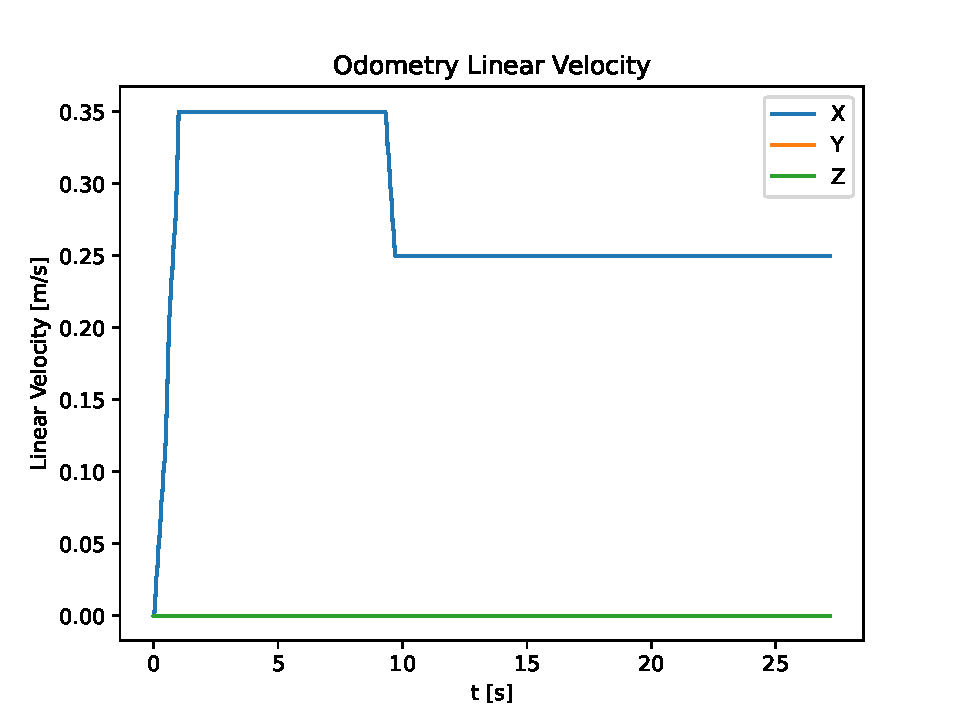
\includegraphics[width=0.5\textwidth]{pics/odometry_linear_velocity.pdf}
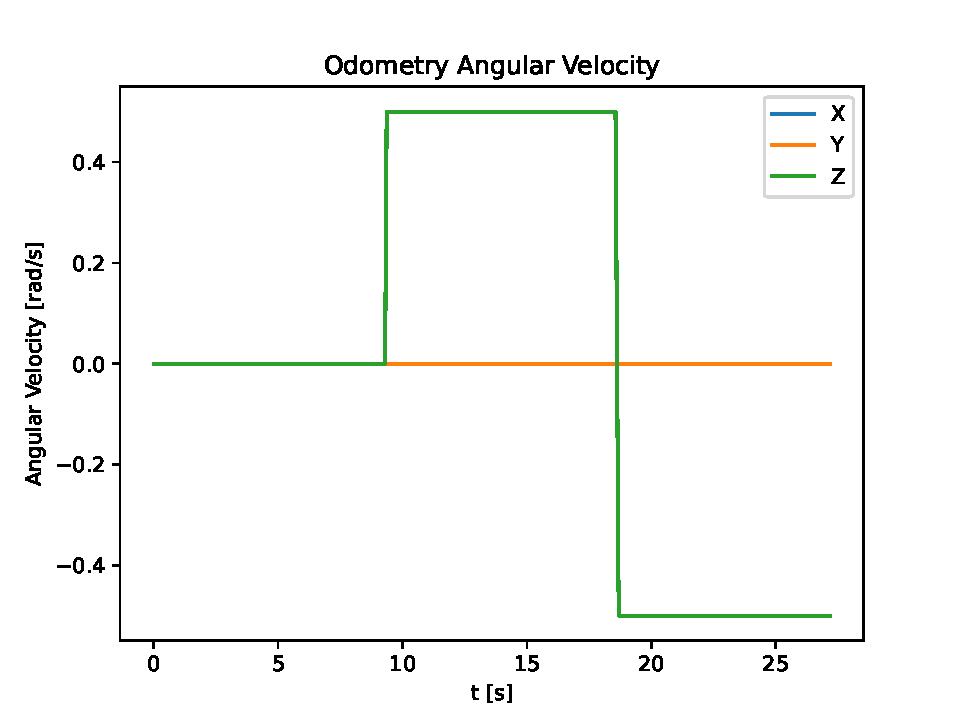
\includegraphics[width=0.5\textwidth]{pics/odometry_angular_velocity.pdf}

Damit ergeben sich folgende Odometriepositionen und -orientierungen:
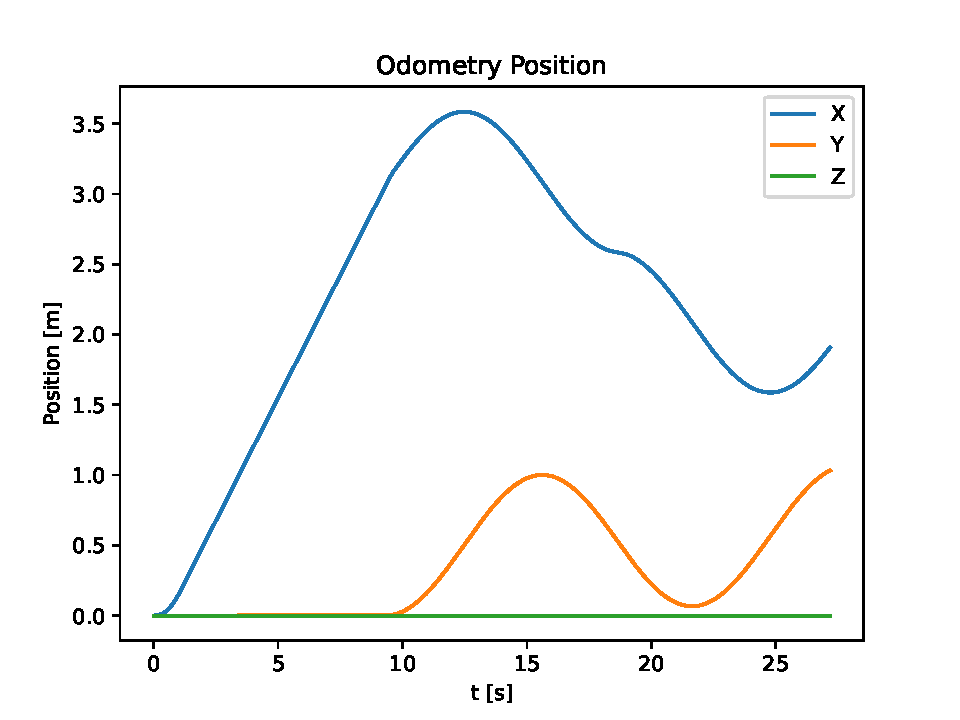
\includegraphics[width=0.5\textwidth]{pics/odometry_position.pdf}
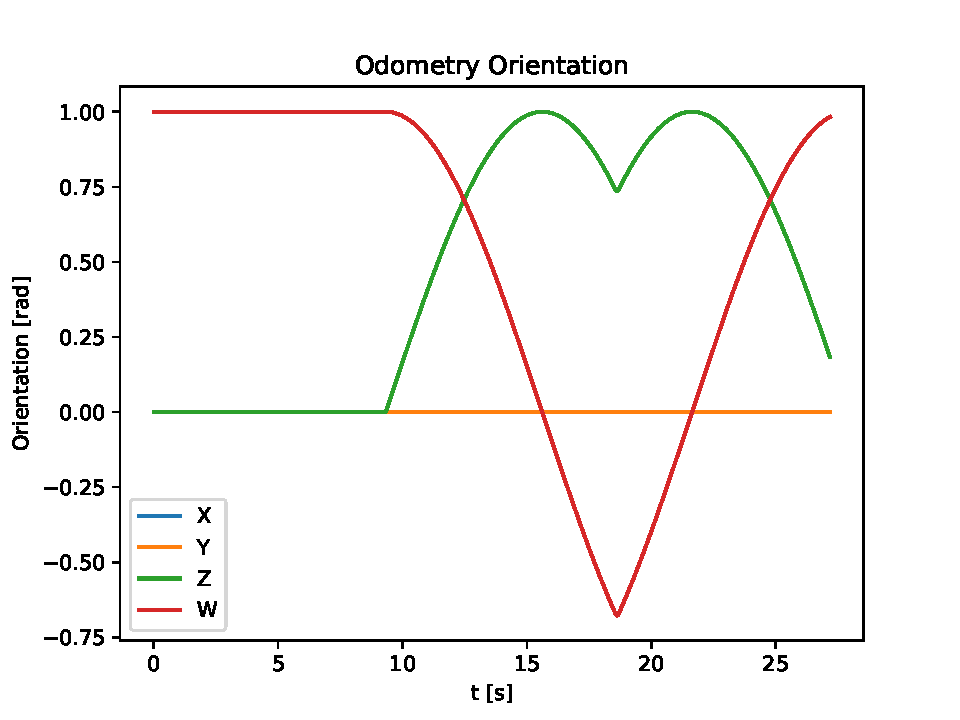
\includegraphics[width=0.5\textwidth]{pics/odometry_orientation.pdf}

In den ersten 10 Ticks bewegt sich der Roboter geradlinig. Da sich die Orientierung nicht ändert, ist auch der Verlauf des Quaternions konstant.
Ab 10 Ticks beginnt der Roboter sich abwechselnd nach links und rechts zu drehen. Aufgrund der Kreisbewegung bewegt sich die X- und Y-Komponente in Form einer Sinuskurve.
Gleichzeitig ändert sich die Orientierung des Roboters.

Wird die Inertial Measurement Unit (IMU) betrachtet, so ergeben sich folgende Messwerte:

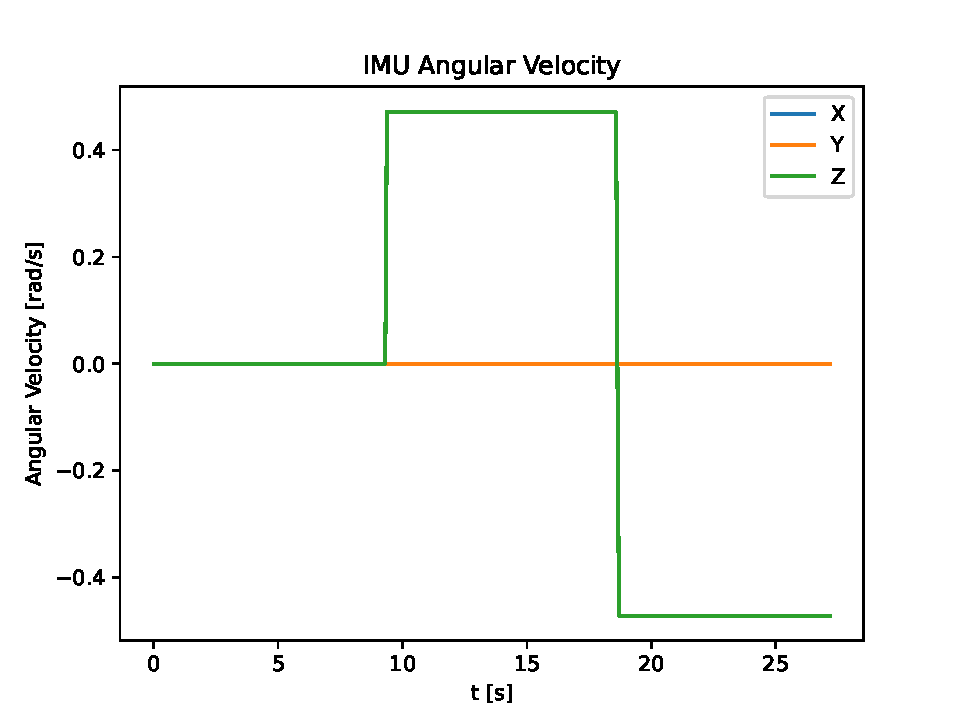
\includegraphics[width=0.5\textwidth]{pics/imu_angular_velocity.pdf}
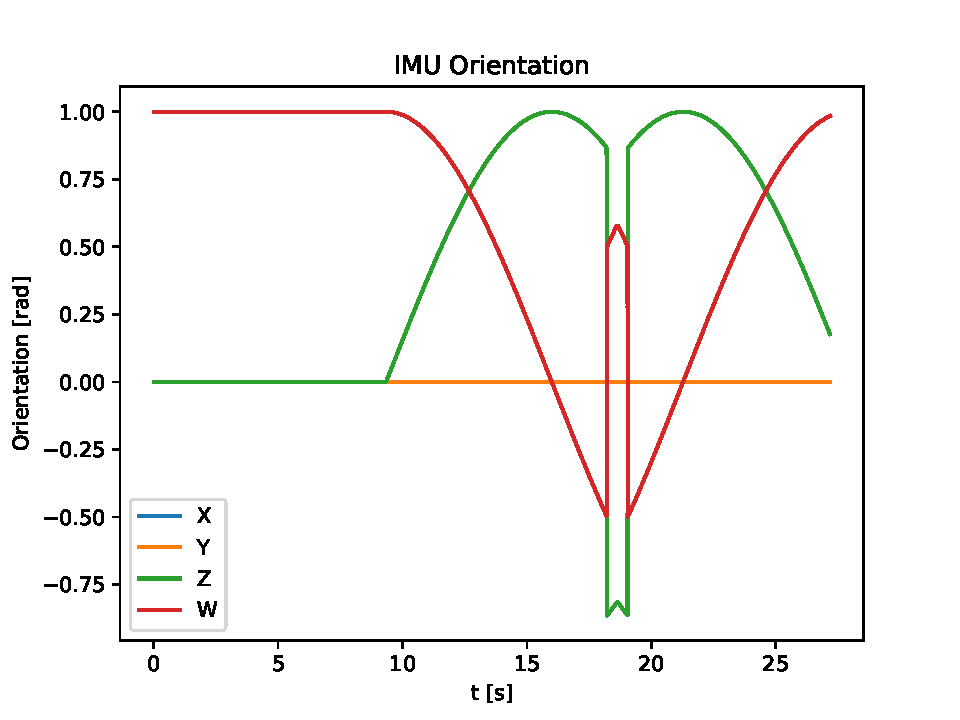
\includegraphics[width=0.5\textwidth]{pics/imu_orientation.pdf}

Die Geschwindigkeit stimmt weitestgehend mit der Odometrie überein. Die Orientierung zeigt jedoch im Vergleich zur Odometrie eine deutliche Unstetigkeit im Bereich bei 20 Ticks.
Es wirkt so als ob das Vorzeichen des Quaternions plötzlich umgekehrt wird.

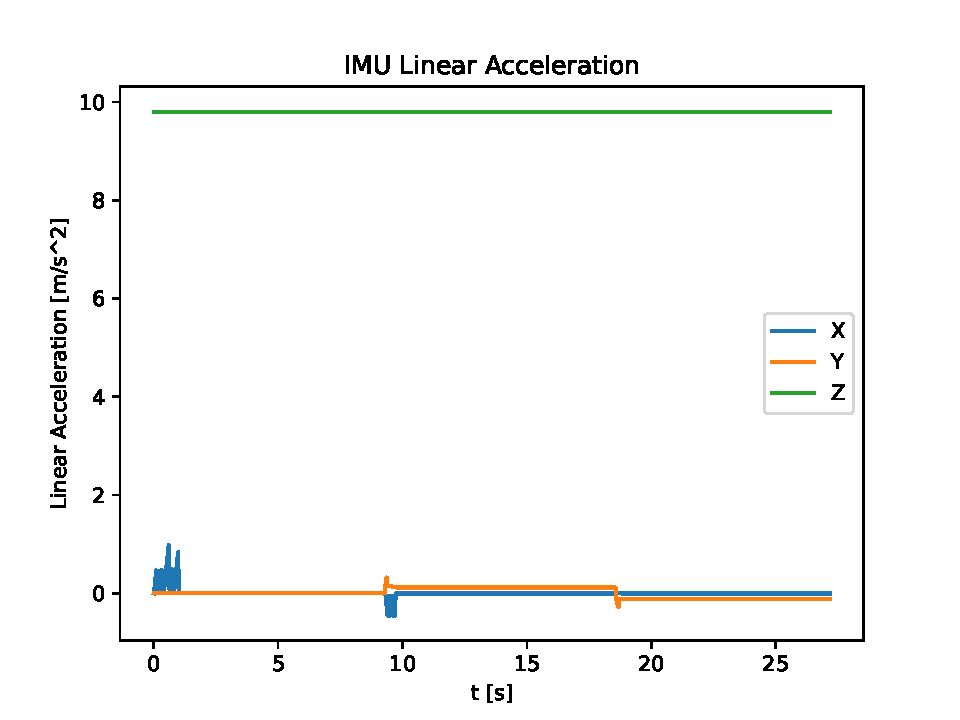
\includegraphics[width=0.5\textwidth]{pics/imu_linear_acceleration.pdf}

Sensorrauschen ist in der Messung der Beschleunigung deutlich zu erkennen. Auch die Gravitationskraft ist
in der Z-Komponente zu erkennen. Der folgende Codeausschnitt zeigt die Implementierung der Bewegungsmodellierung:

\lstinputlisting[
    language=Python,
    caption={Code zur Bewegungsmodellierung},
    label={lst:bewegungsmodellierung},
]{../p1a.py}

\chapter{Inertial navigation}

\chapter{Sensoren in XACRO}

Der Roboter verfügt über zwei Sensoren. In diesem Abschnitt wird der vordere Sensor in seiner relativen Position zum Roboter
nach oben verschoben, so dass er auch die Tischplatte erkennen kann.
Folgende Abbildungen zeigen diese Verschiebung durch die Modifizierung der Z-Komponente des Sensors in der XACRO-Datei.

\begin{figure}
    \centering
    \begin{minipage}{0.45\textwidth}
        \centering
        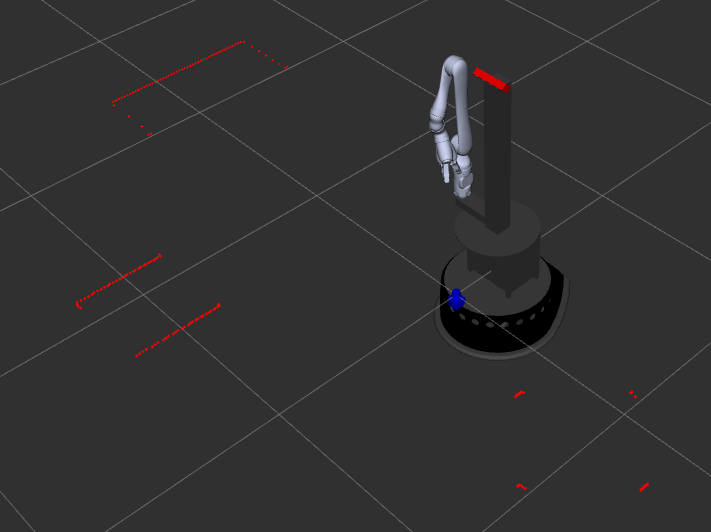
\includegraphics[width=\linewidth]{pics/robo_low.png}
        \caption{Niedrige Sensorstellung}

    \end{minipage}\hfill
    \begin{minipage}{0.45\textwidth}
        \centering
        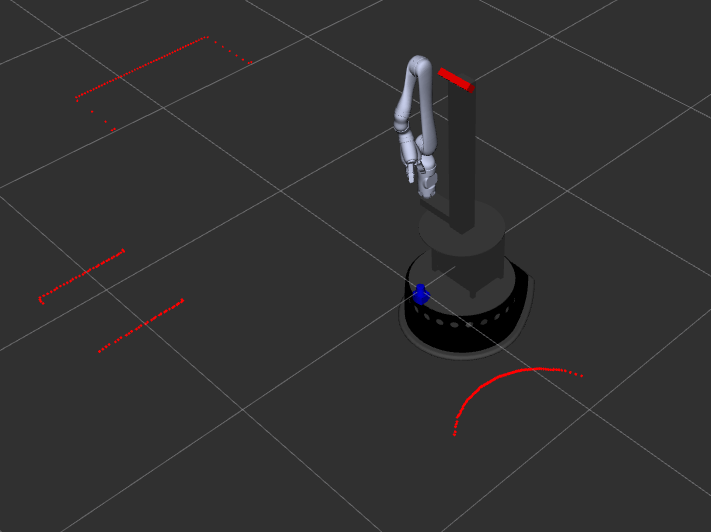
\includegraphics[width=\linewidth]{pics/robo_high.png}
        \caption{Hohe Sensorstellung}
    \end{minipage}

\end{figure}

\chapter{Robert as vacuum cleaner}

\chapter{Koordinatentransformation}
Ein Roboter mit den Weltkoordinaten (Translationsvektor) \(\boldsymbol{\tau}^w = \begin{pmatrix} 5 & 3 & 0 \end{pmatrix}^{T}\)
wird um die z-Achse gedreht. Damit ergibt sich die Rotationsmatrix \(\mathbf{C}^r_w\) von Welt- zu Roboterkoordinaten, die
abhängig vom Winkel \(\theta\) ist.


\[
    \mathbf{C}^r_w(\theta) =
    \begin{pmatrix}
        \cos\theta  & \sin\theta & 0 \\
        -\sin\theta & \cos\theta & 0 \\
        0           & 0          & 1
    \end{pmatrix}
\]
Wird nun ein Objekt in den Weltkoordinaten \(\mathbf{v}^w = \begin{pmatrix} 9 & 1 & 1 \end{pmatrix}^{T}\) betrachtet,
so kann dessen Position in den Roboterkoordinaten \(\mathbf{v}^r\) durch folgende Gleichung berechnet werden:

\[
    \mathbf{v}^r = \mathbf{C}^r_w(\mathbf{v}^w - \boldsymbol{\tau}^w)
\]

In homogenen Koordinaten kann dies auch durch die folgende Gleichung berechnet werden:

\[
    \tilde{\mathbf{v}}^r =
    \begin{pmatrix}
        \mathbf{v}^r \\
        1
    \end{pmatrix}
    =
    \begin{pmatrix}
        \mathbf{C}^r_w & -\mathbf{C}^r_w\boldsymbol{\tau}^w \\
        0              & 1
    \end{pmatrix}
    \tilde{\mathbf{v}}^w
\]

Mit dem Winkel \(\theta = \frac{\pi}{6}\) ergibt sich:

\[
    \tilde{\mathbf{v}}^r = \begin{pmatrix}
        \frac{\sqrt{3}}{2} & 0.5                & 0 & -5.83013 \\
        -0.5               & \frac{\sqrt{3}}{2} & 0 & -0.09808 \\
        0                  & 0                  & 1 & 0        \\
        0                  & 0                  & 0 & 1
    \end{pmatrix}
    \begin{pmatrix}
        9 \\ 1 \\ 1 \\ 1
    \end{pmatrix}
    =
    \begin{pmatrix}
        2.46410 \\ -3.73205 \\ 1 \\ 1
    \end{pmatrix}
\]

In inhomogenen Koordinaten ergibt sich somit:

\[\mathbf{v}^r = \begin{pmatrix} 2.46 & -3.73 & 1 \end{pmatrix}^{T}\]

Wird hingegen der Punkt \(\mathbf{u}^r = \begin{pmatrix} 1 & 0 & 0 \end{pmatrix}^{T}\) in den Roboterkoordinaten betrachtet, so kann dessen Position in den Weltkoordinaten \(\mathbf{u}^w\) durch folgende Gleichung berechnet werden:

\[
    \mathbf{u}^w = \mathbf{C}^w_r\mathbf{u}^r + \boldsymbol{\tau}^w
\]

In homogenen Koordinaten ergibt sich somit:

\[
    \tilde{\mathbf{u}}^w =
    \begin{pmatrix}
        \mathbf{C}^w_r & \boldsymbol{\tau}^w \\
        0              & 1
    \end{pmatrix}
    \tilde{\mathbf{u}}^r
\]

Mit dem Winkel \(\theta = \frac{\pi}{6}\) und der Relation \(\mathbf{C}^w_r = (\mathbf{C}^r_w)^T\) ergibt sich:

\[
    \tilde{\mathbf{u}}^w = \begin{pmatrix}
        \frac{\sqrt{3}}{2} & -0.5               & 0 & 5 \\
        0.5                & \frac{\sqrt{3}}{2} & 0 & 3 \\
        0                  & 0                  & 1 & 0 \\
        0                  & 0                  & 0 & 1
    \end{pmatrix}
    \begin{pmatrix}
        1 \\ 0 \\ 0 \\ 1
    \end{pmatrix}
    =
    \begin{pmatrix}
        5.86603 \\ 3.5 \\ 0 \\ 1
    \end{pmatrix}
\]

Damit ergibt sich in inhomogenen Koordinaten:

\[\mathbf{u}^w = \begin{pmatrix} 5.87 & 3.5 & 0 \end{pmatrix}^{T}\]

\chapter{Sensorrauschen}

Beschleunigungssensoren sind ständigem (weißen) Rauschen \(w_t\) ausgesetzt. Die Verteilung des integrierten Rauschens (Geschwindigkeitsrauschen) \(B_t = \int_0^t w_\tau d\tau\) kann durch folgende Gleichung beschrieben werden:

\[
    B_t \sim \mathcal{N}(\mu, \sigma^2) \quad \text{mit} \quad \mu = 0 \frac{m}{s} \quad \text{und} \quad \sigma^2 c \times t = 5 \frac{m^2}{s^2}
\]

Man spricht auch von Brownscher Bewegung mit der Konstanten \(c = 5 \frac{m^2}{s^3}\). Im Gegensatz zu einem konstanten Bias \(b\) ist die Varianz des weißen Rauschens zeitabhängig.

Nach einer Zeit von \(t=5s\) ergibt sich somit eine Varianz von \(\sigma^2 = c \times t = 5 \frac{m^2}{s^3} \times 5s = 25 \frac{m^2}{s^2}\) und damit eine Verteilung von:

\[
    B_t \sim \mathcal{N}(0, 25) \quad \text{mit} \quad \sigma = 5 \frac{m}{s}
\]

\clearpage
\printbibliography[heading=bibintoc]

\end{document}